%\documentclass[a4paper, 12pt]{scrreprt}

\documentclass[a4paper, 12pt]{scrartcl}
%usepackage[german]{babel}
\usepackage{microtype}
%\usepackage{amsmath}
%usepackage{color}
\usepackage[utf8]{inputenc}
\usepackage[T1]{fontenc}
\usepackage{wrapfig}
\usepackage{lipsum}% Dummy-Text
\usepackage{multicol}
\usepackage{alltt}
%%%%%%%%%%%%bis hierhin alle nötigen userpackage
\usepackage{tabularx}
\usepackage[utf8]{inputenc}
\usepackage{amsmath}
\usepackage{amsfonts}
\usepackage{amssymb}

%\usepackage{wrapfig}
\usepackage[ngerman]{babel}
\usepackage[left=25mm,top=25mm,right=25mm,bottom=25mm]{geometry}
%\usepackage{floatrow}
\setlength{\parindent}{0em}
\usepackage[font=footnotesize,labelfont=bf]{caption}
\numberwithin{figure}{section}
\numberwithin{table}{section}
\usepackage{subcaption}
\usepackage{float}
\usepackage{url}
%\usepackage{fancyhdr}
\usepackage{array}
\usepackage{geometry}
%\usepackage[nottoc,numbib]{tocbibind}
\usepackage[pdfpagelabels=true]{hyperref}
\usepackage[font=footnotesize,labelfont=bf]{caption}
\usepackage[T1]{fontenc}
\usepackage {palatino}
%\usepackage[numbers,super]{natbib}
%\usepackage{textcomp}
\usepackage[version=4]{mhchem}
\usepackage{subcaption}
\captionsetup{format=plain}
\usepackage[nomessages]{fp}
\usepackage{siunitx}
\sisetup{exponent-product = \cdot, output-product = \cdot}
\usepackage{hyperref}
\usepackage{longtable}
\newcolumntype{L}[1]{>{\raggedright\arraybackslash}p{#1}} % linksbündig mit Breitenangabe
\newcolumntype{C}[1]{>{\centering\arraybackslash}p{#1}} % zentriert mit Breitenangabe
\newcolumntype{R}[1]{>{\raggedleft\arraybackslash}p{#1}} % rechtsbündig mit Breitenangabe
\usepackage{booktabs}
\renewcommand*{\doublerulesep}{1ex}
\usepackage{graphicx}



\begin{document}

\section {Auswertung}

Zur genauen Bestimmung, der Relation zwischen der Gitterpositionsspannung und der Wellenzahl wurde das Licht einer Natriumdampflampe an dem verwendeten Czerny-Turner-Monochromators gebeugt und das Spektum der nullten \ref{Null} und ersten \ref{Eins} Ornung aufgenommen. 


\begin{figure}[H]
	\centering	
	\begin{minipage}{1\textwidth}
	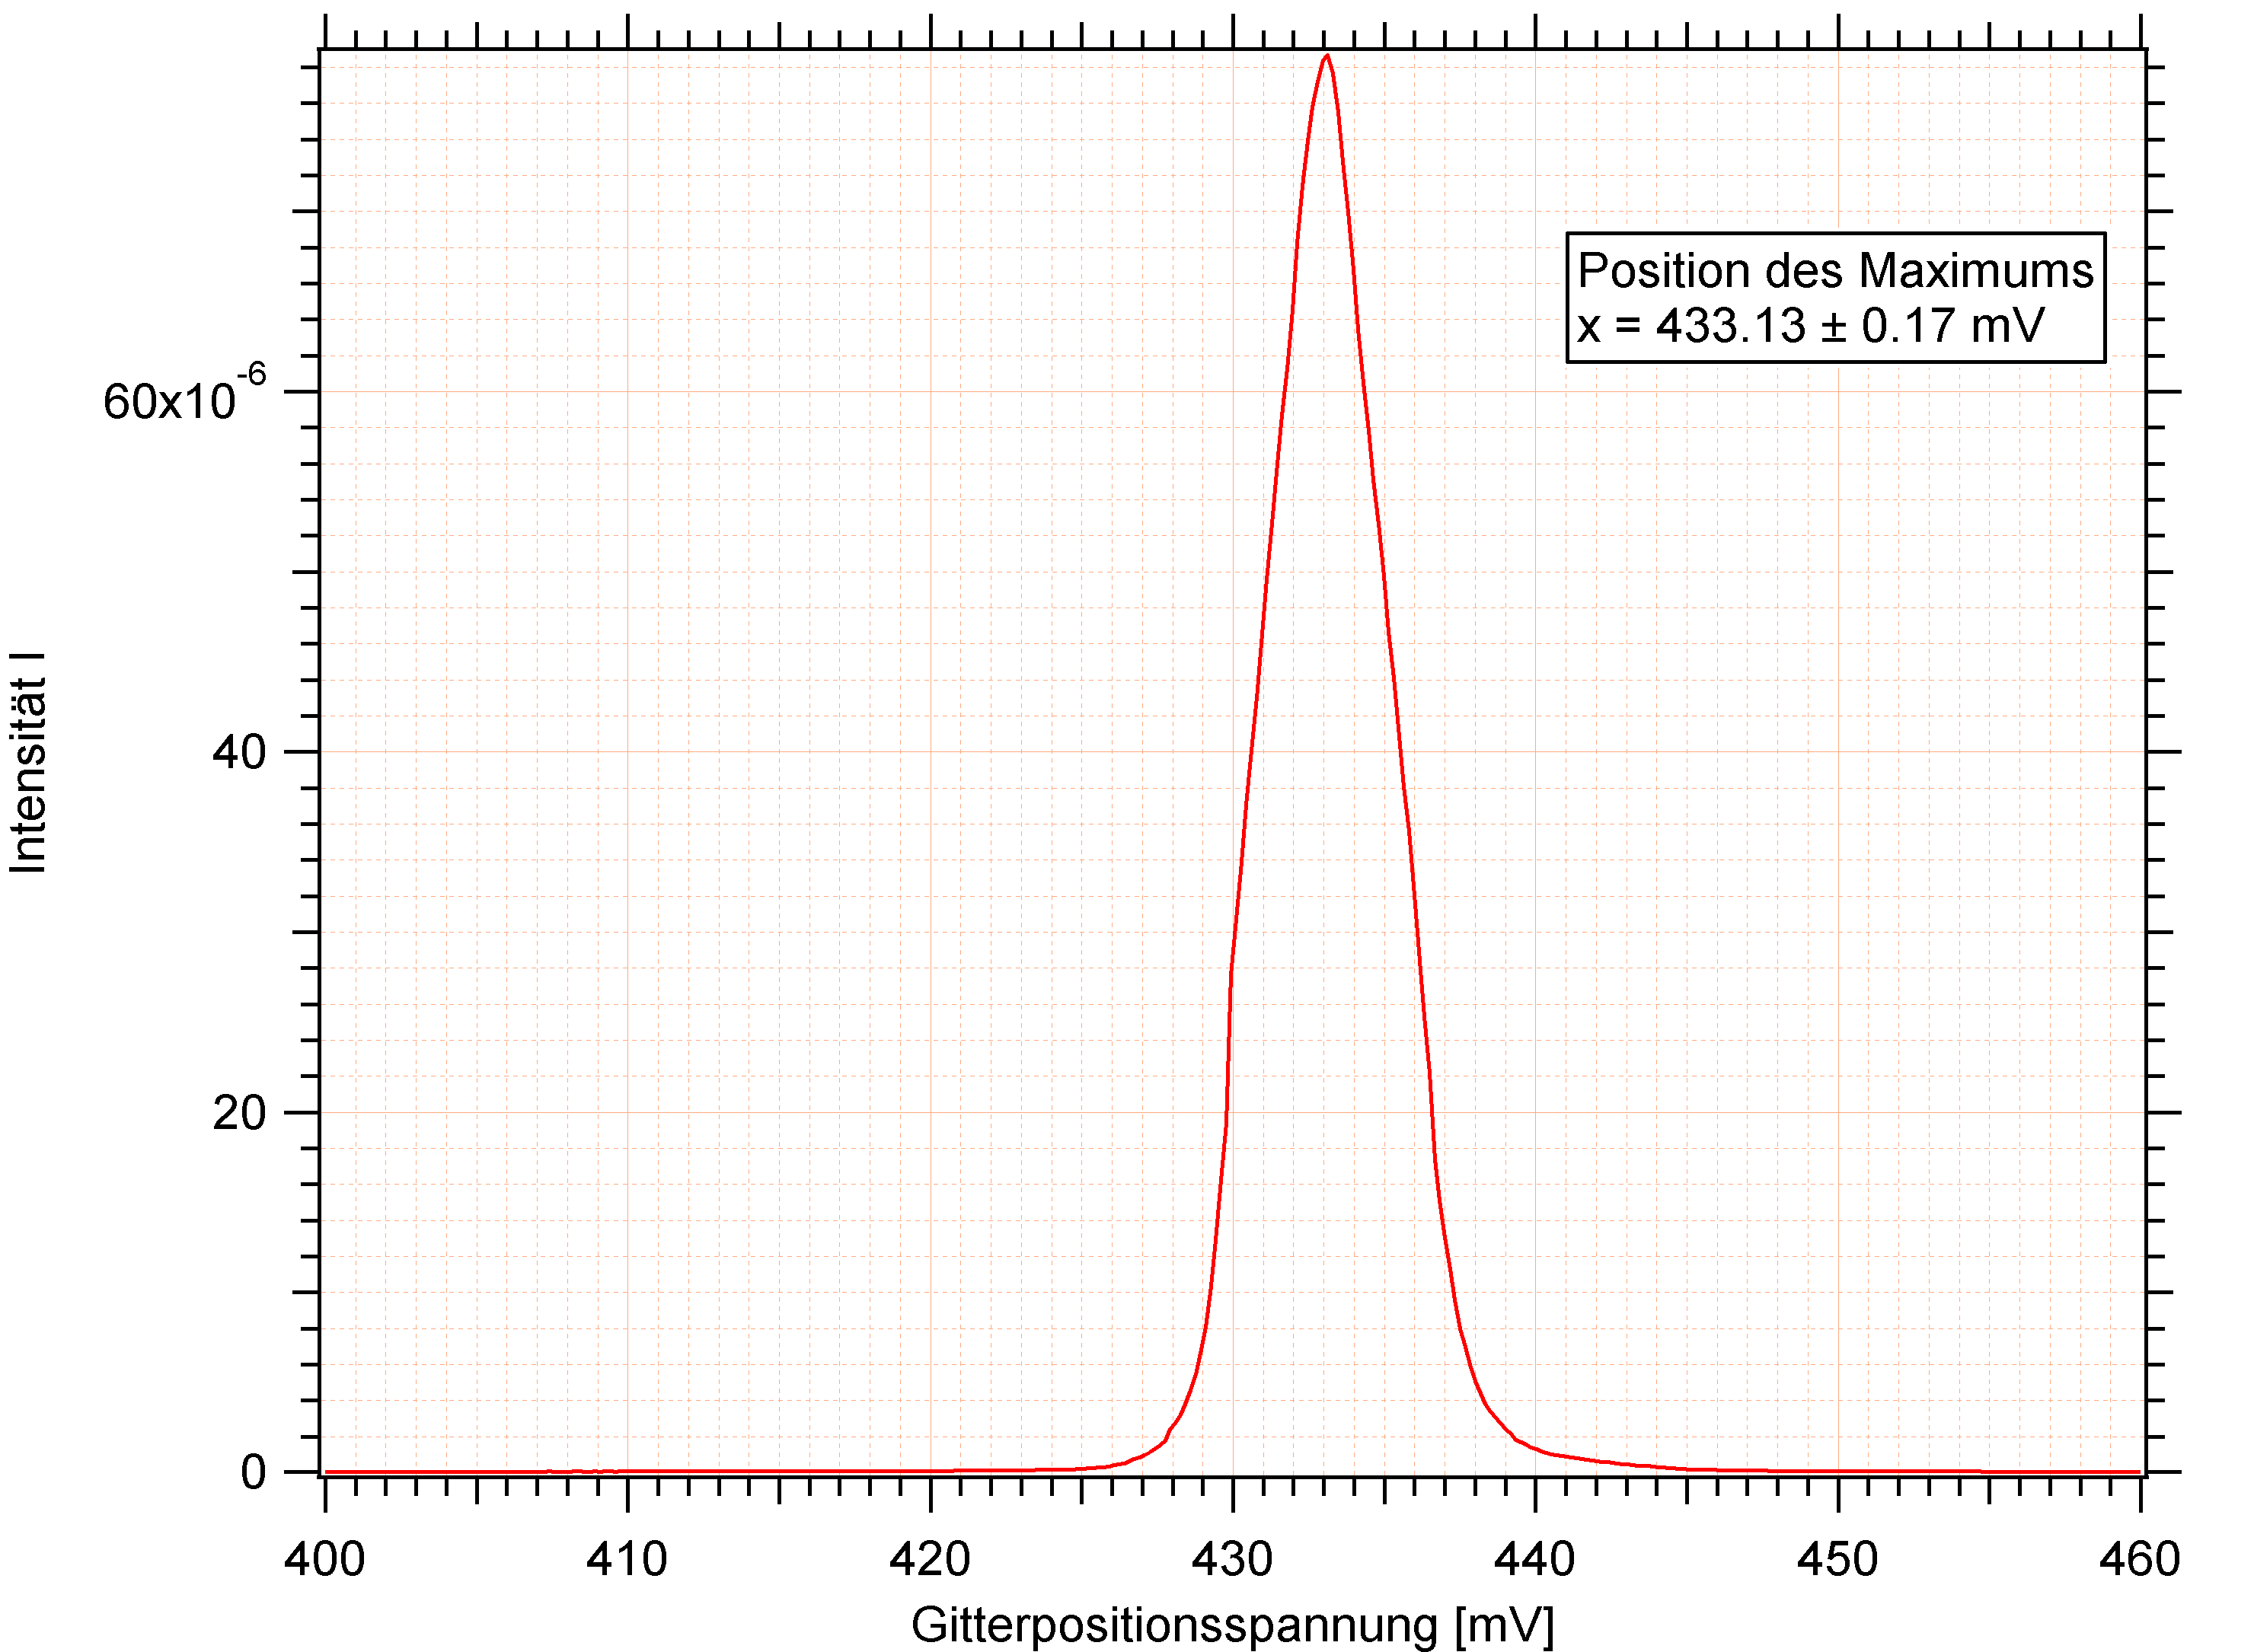
\includegraphics[width=\columnwidth]{Bilder/Graph1.png}
	\end{minipage}
	
	
	\caption{Emissionsspektrum einer Natriumdampflampe bei der nullten Ordnung}
	

	\label{Null}
\end{figure}
%%%%%%%%%%%%%%%%%%%%%%%%%%%	
\begin{figure}[H]
	\centering	
	\begin{minipage}{1\textwidth}
	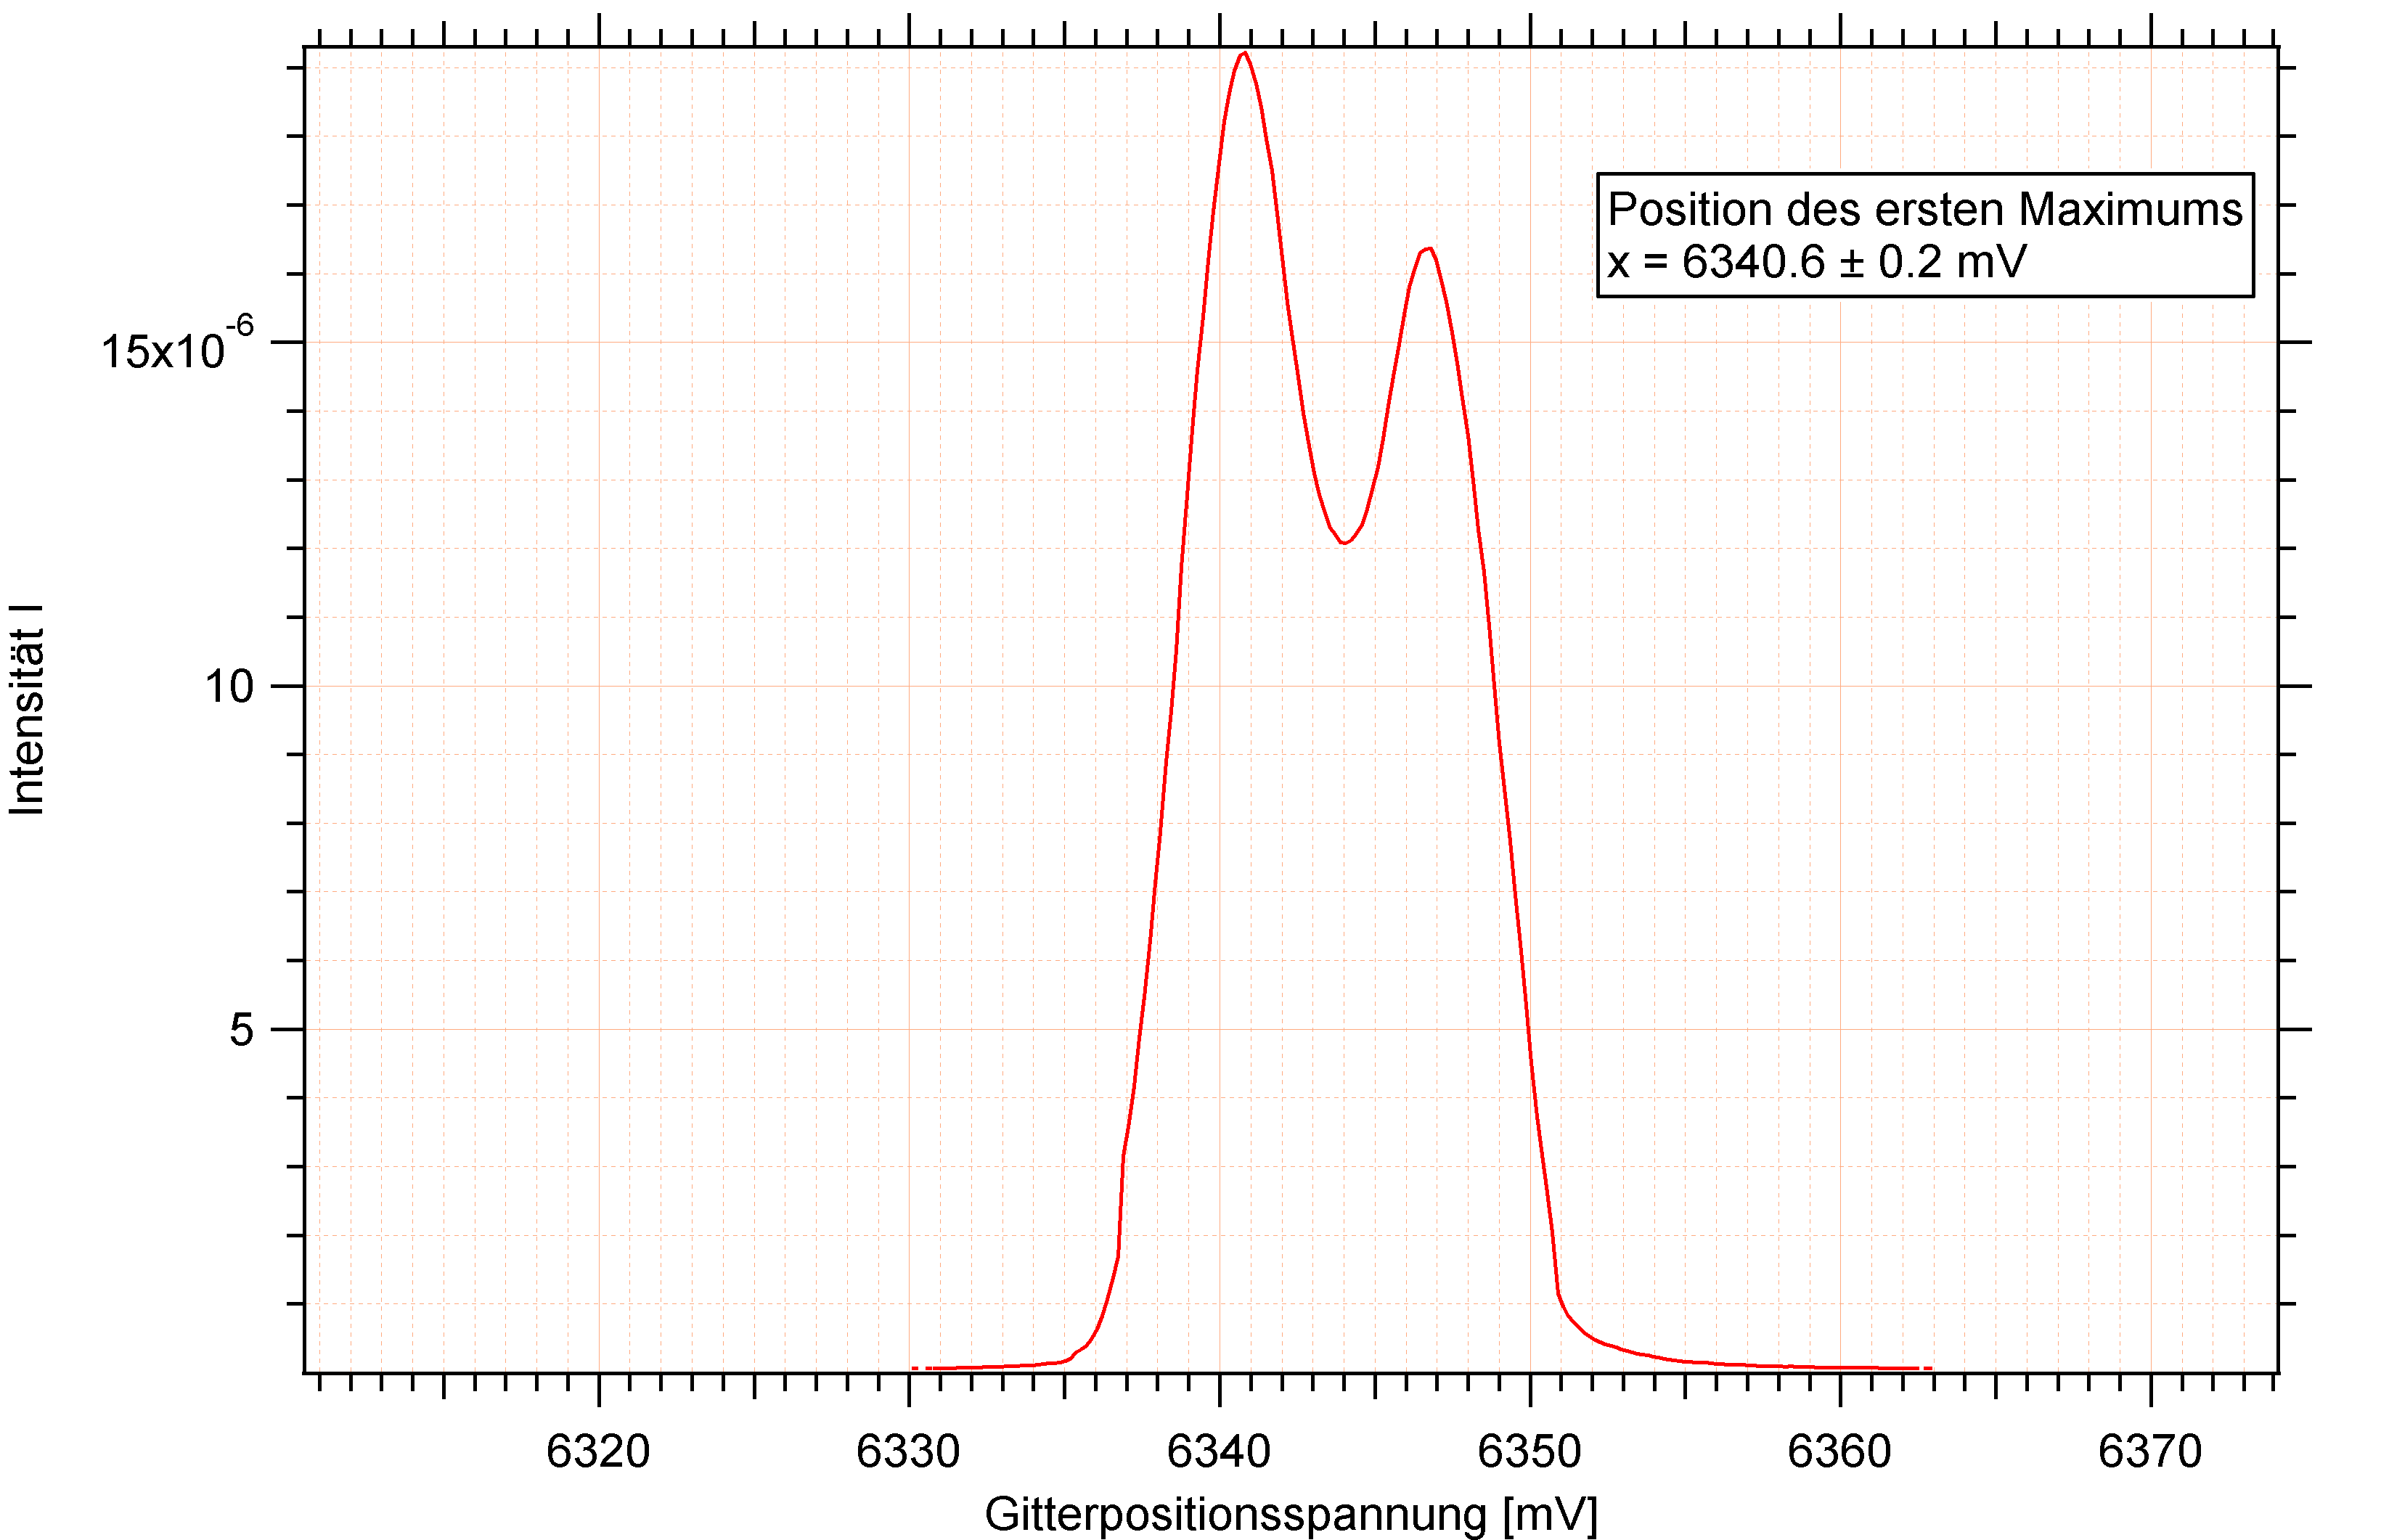
\includegraphics[width=\columnwidth]{Bilder/Graph2.png}
	\end{minipage}
	
	
	\caption{Emissionsspektrum einer Natriumdampflampe bei der ersten Ornung.}
	
	
	\label{Eins}
\end{figure}



Da die Wellenlängen der Natrium-D-Linien hinreichend bekannt sind, ist es möglich aus der Spannung, die mit der Position des Gitters korreliert, die Änderung der Wellenlänge pro Spannungsänderung zu berechnen. Außerdem wurde durch die Spannung beim Peak der nullten Ordnung die Verschiebung der Wellenlängenskala zur Sannungsskala bestimmt.

\begin {equation}
\frac{dU}{d\lamda}=\frac{\Delta U}{\Delta\lamda}=\frac{6340.6 mV - 433.13 mV}{588.995 nm}=10.03 \frac{mV}{nm}
\end {equation}


Auf dieser Grundlage wurde das Emissionsspektrum \ref{Bunsen} einer rauschenden Bunsenbrennerflamme aufgenommen, welche mit Butan betrieben wurde. Die augnommenen Peaks stammen aus der Relaxation des elektronisch angeregtem C2-Radikal.



\begin{figure}[H]
	\centering	
	\begin{minipage}{1\textwidth}
	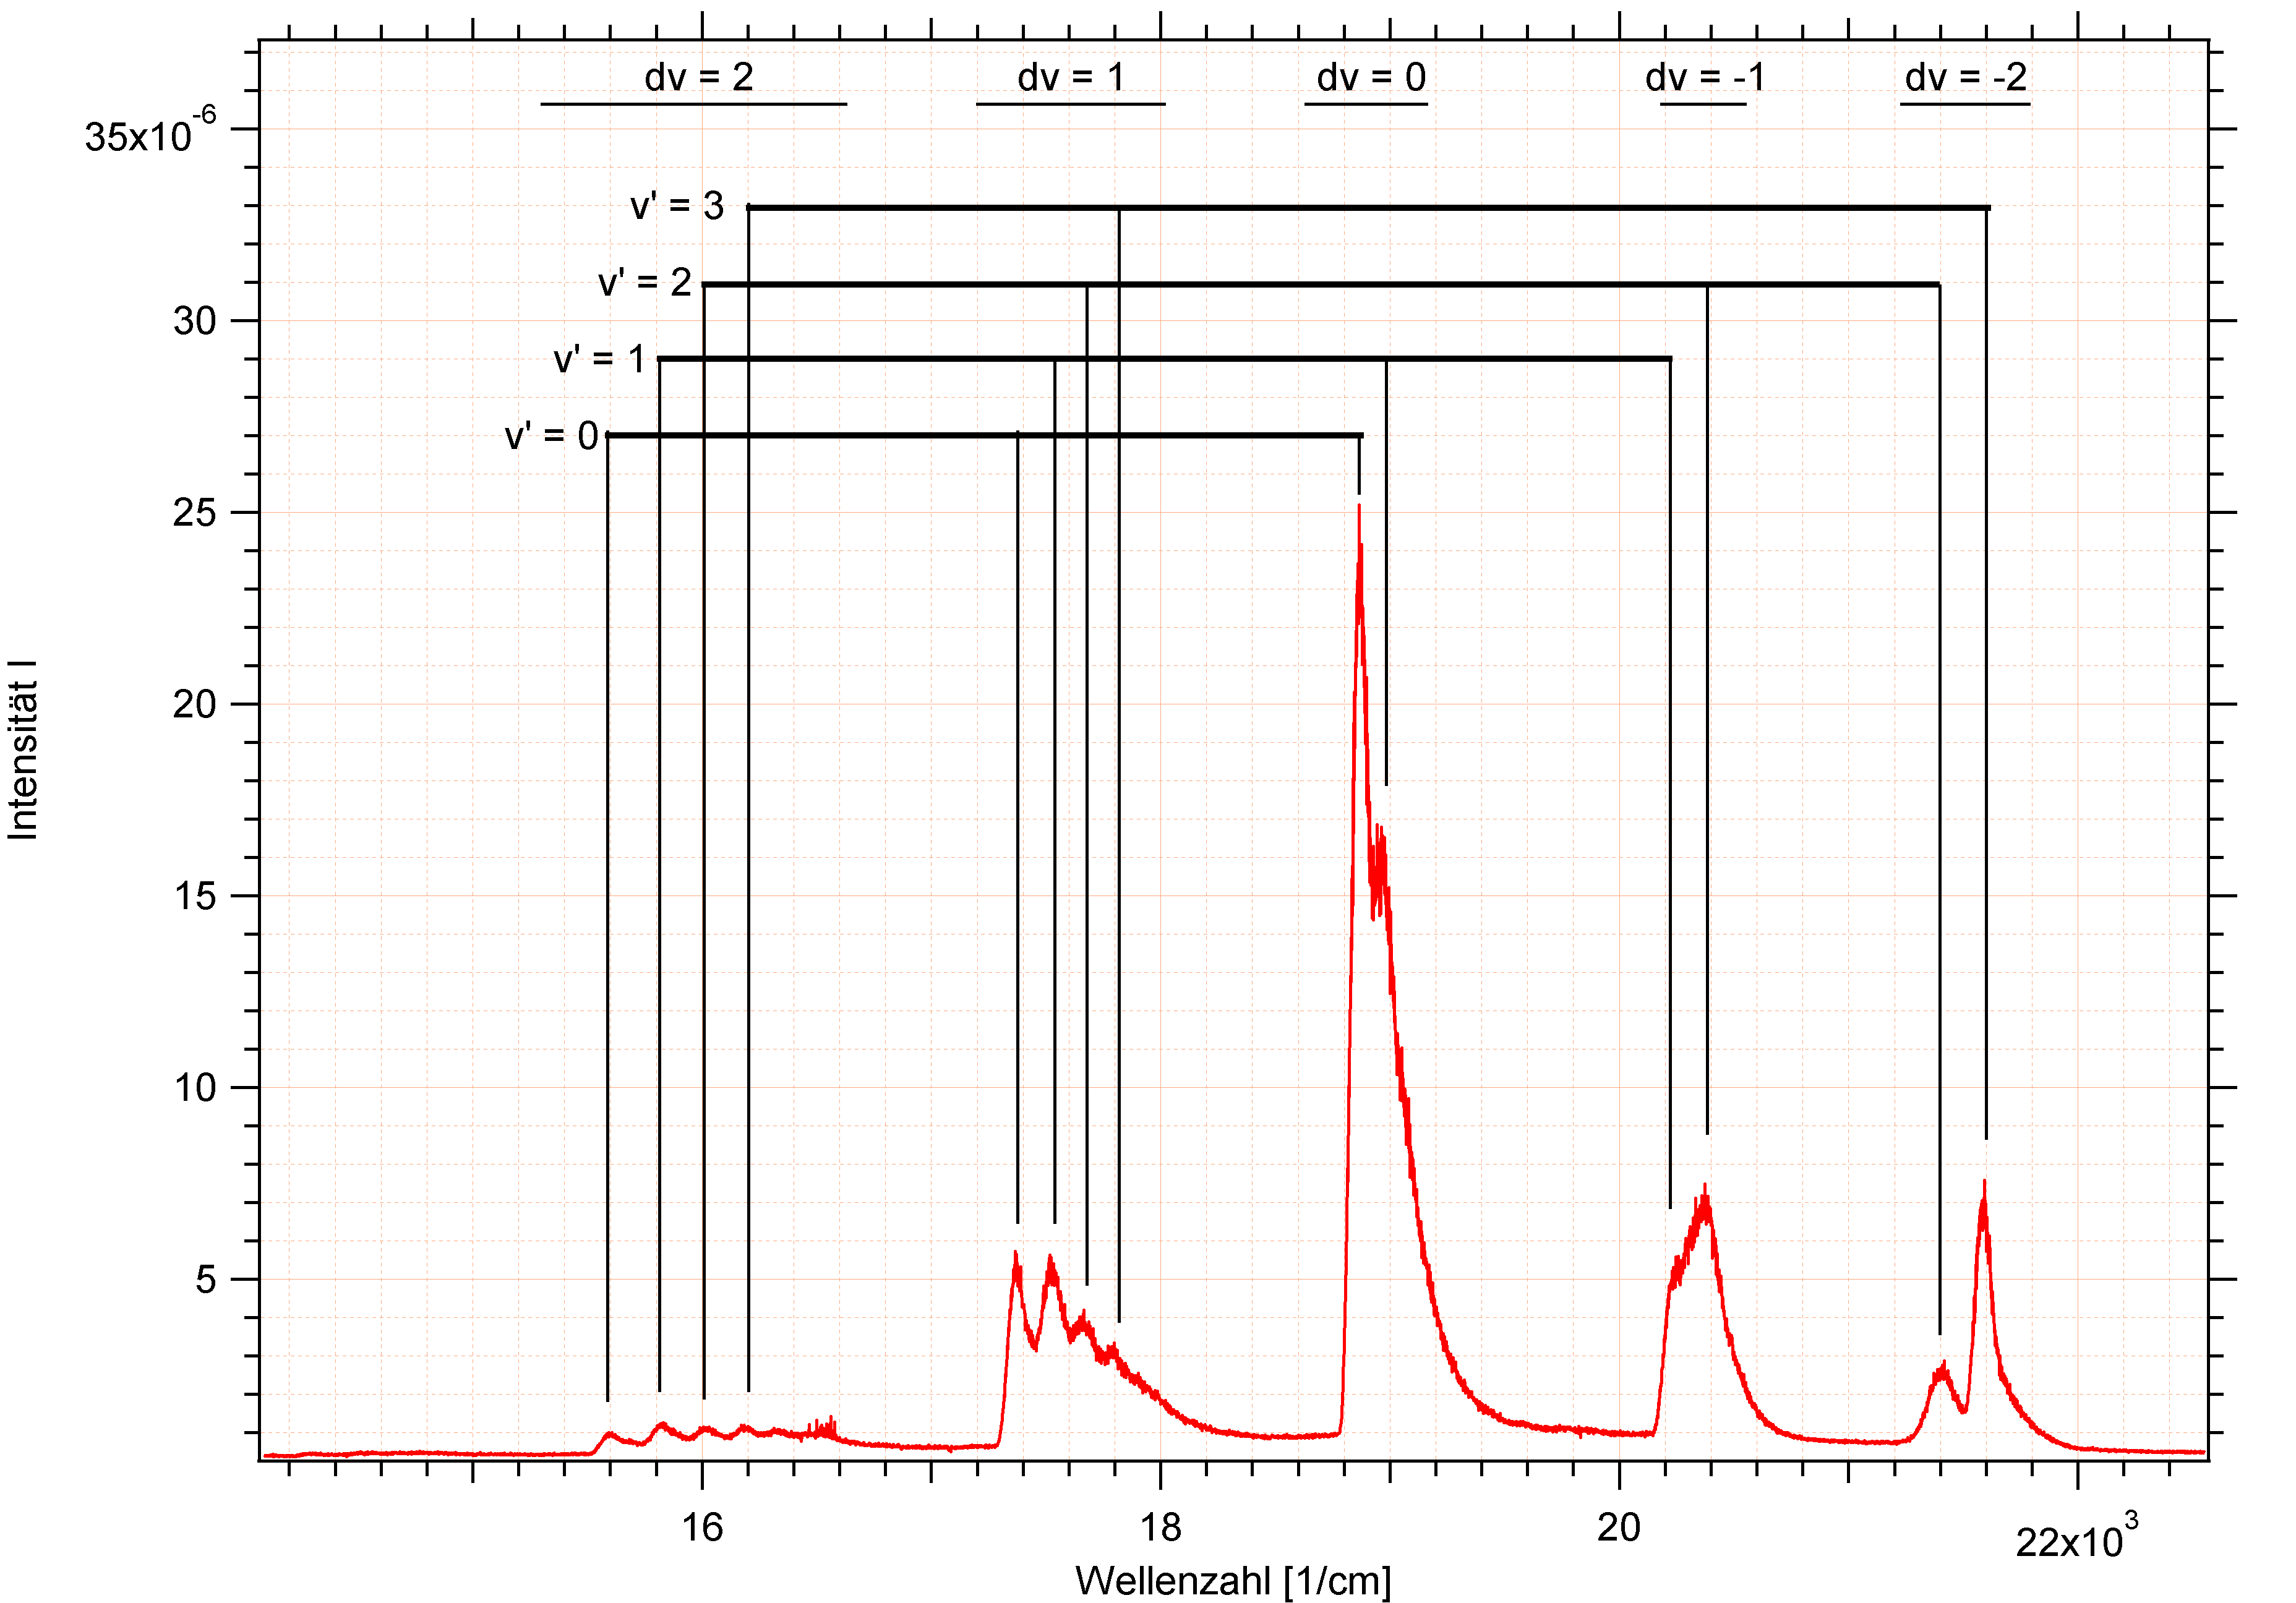
\includegraphics[width=\columnwidth]{Bilder/Graph3.png}
	\end{minipage}
	
	
	\caption{Emissionsspektrum der Bunsenbrennerflamme.}
	

	\label{Bunsen}
\end{figure}

Durch die Benennung einiger markanter Banden war es möglich mit einer Fitfunktion \nu_e, die harmonischen Schwingungskonstanten und die anharmonizitätskonstanten des Grund-, und Angeregtenzustandes berechen, welche in Tabelle  \ref{tab1} zusammengefasst sind.


\begin{table}[H]

 
 
 \caption{Ergebnisse des Fits  }
\begin{tabular}{L{0.1\linewidth}L{0.1\linewidth}L{0.15\linewidth}R{0.05\linewidth}L{0.2\linewidth}L{0.25\linewidth}}

 
 Konstante&  &  Messwert & &  Literatur \cite{Lit} \\
  \addlinespace[1ex]
\hline
\addlinespace[1ex]
  {\nu}_e  & $\tilde{\nu}_e $&\SI[mode=math]{1968.5}{cm^{-1}}  \\
 {\omega}'_e & $\tilde{\nu}_e x_e$& \SI[mode=math]{13.91}{cm^{-1}}&$\pm$ &\SI[mode=math]{0.05}{cm^{-1}}&\SI[mode=math]{13.28831}{cm^{-1}} \\
  {\omega}'_e x'_e& $r_e$&\SI[mode=math]{11.7000e-9}{cm} & $\pm$ &\SI[mode=math]{0.0003e-9}{cm}&\SI[mode=math]{11.28323e-9}{cm}\\
  {\omega}''_e  & $D_e$&\SI[per-mode=fraction]{833}{\kJ\per\mol} &$\pm$ &\SI[per-mode=fraction]{7}{\kJ\per\mol}&\SI[per-mode=fraction]{729}{\kJ\per\mol} \\
   {\omega}''_e x''_e&$B$&	\SI[mode=math]{2}{cm^{-1}}&$\pm$ &\SI[mode=math]{1}{cm^{-1}}&\SI[mode=math]{1.93128087}{cm^{-1}}\\
\addlinespace[1ex]
\hline
\addlinespace[1ex]
  HCl  & $\tilde{\nu}_e$ &\SI[mode=math]{2654}{cm^{-1}} &$\pm$ &\SI[mode=math]{1}{cm^{-1}} &\SI[mode=math]{2990.946}{cm^{-1}} \\
  HCl  & $\tilde{\nu}_e x_e$& \SI[mode=math]{60.0}{cm^{-1}}&$\pm$ &\SI[mode=math]{0.5}{cm^{-1}}&\SI[mode=math]{52.8186}{cm^{-1}} \\
  HCl  & $r_e$&\SI[mode=math]{13.3333e-9}{cm} & $\pm$ &\SI[mode=math]{0.0008e-9}{cm}&\SI[mode=math]{12.7455e-8}{cm}\\
  HCl  & $D_e$&\SI[per-mode=fraction]{351}{\kJ\per\mol} &$\pm$ &\SI[per-mode=fraction]{5}{\kJ\per\mol}&\SI[per-mode=fraction]{429}{\kJ\per\mol} \\
    HCl&$B$&	\SI[mode=math]{13.00}{cm^{-1}}& $\pm$ & \SI[mode=math]{7.5}{cm^{-1}}&\SI[mode=math]{10.59341}{cm^{-1}}\\
\addlinespace[1ex]
\hline   
   
 \end{tabular}
 \label{tab1}
 \end{table}


